\section{Teori}
I boken ''Software Product Quality Control'' \cite{SPQC} nämns ett antal definitioner som förtydligar vad kvalitetssäkring innebär, dessa syns nedan.  

\begin{itemize}
  \item ''Quality assurance: a planned and systematic pattern of all actions necessary to provide adequate confidence that an item or product conforms to established technical requirements.'' 
  \item ''Constructive quality assurance: All means to be used in constructing a product in a way so it meets its quality requirements.'' 
  \item ''Analyctical quality assurance: All means of analysing the state of the quality of a product.'' 
\end{itemize}
\noindent Kvalitetssäkring innebär följaktligen att man som leverantör av en produkt eller tjänst ska se till att de uppfyller de krav som har satts upp i en eventuell kravspecifikation. Att man under arbetsgången analyserar om man är på väg att uppfylla kraven eller inte, i sådana fall måste detta åtgärdas omedelbart.
\newline
\newline
Med detta sagt finns det flera steg i ett projekt att kvalitetssäkra. Ett effektivt sätt att göra detta på är genom att följa Shewhart cykeln, det vill säga planera, göra, studera och agera (PGSA) \citep{PDCA}. Shewhart cykeln är en iterativ fyra stegs metod, se figur \ref{fig:shewcycle} och metoden är utvecklad av William Edwards Deming. Namnet ''Shewhart'' kommer från en av Demings kollegor \citep[p.~88]{Deming}. 
\begin{figure}[h]
\centerline{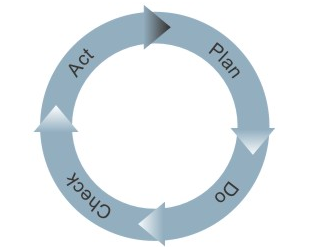
\includegraphics[scale=0.5]{ruben-tex/graphic/shewhartcycle}}
\caption{Shewhart cykeln \citep{Mindtools}}
\label{fig:shewcycle}
\end{figure}
\begin{enumerate}
  \item Planera. I detta skede ska målet fastställas, det vill säga sätta upp de krav som behövs för att kunden skall bli nöjd. Genom att göra detta är det tydligt om vad som skall göras och en överenskommelse finns mellan kund och leverantör. 
  \item Göra. När man väl har fått för sig om vad som behövs göras för att kunden skall bli nöjd är det dags att implementera ett sätt att jobba och fullfölja processen.
  \item Studera. Efter att ha följt processen under en viss period är det dags att utvärdera om processen man har följt kommer leda till att man uppfyller de målen man har fastställt i ''planera''-skedet.
  \item Agera. Om man under ''studera''-skedet upptäcker att processen man följer inte kommer leda till att man uppfyller de krav som kund och leverantör var överens om måste detta åtgärdas omedelbart genom att planera om arbetsprocessen eller i viss mån diskutera kraven med kunden. Om processen som följs kommer uppfylla de krav som har satts upp kan man fortsätta med iterationerna av Shewhart cykeln precis som innan.
\end{enumerate}
\begin{figure}[h]
\centerline{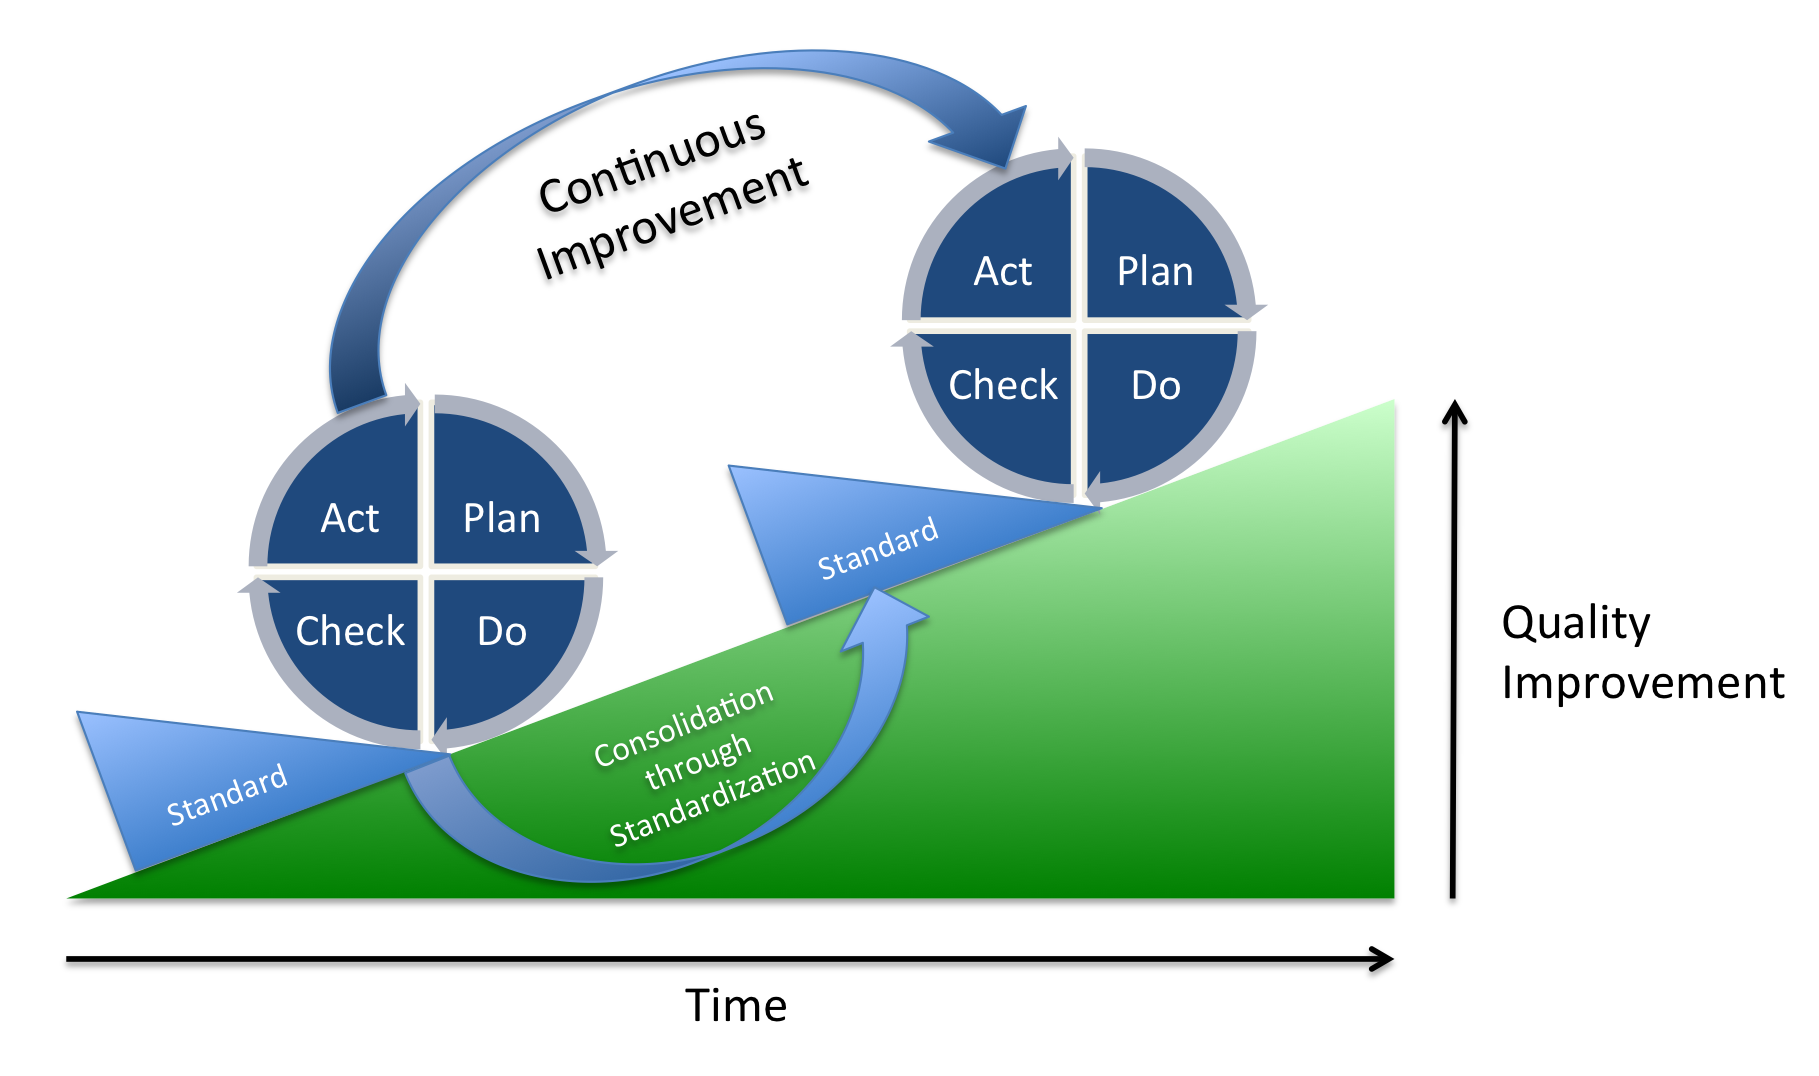
\includegraphics[scale=0.15]{ruben-tex/graphic/PDCA_Process}}
\caption{PDCA process \citep{Vietze}}
\label{fig:pdcaprocess}
\end{figure}
\noindent Genom att följa Shewhart cykeln under ett projekt kan man iterativt förbättra sin arbetsprocess och genom detta öka kvaliteten av den produkt man utvecklar, se figur \ref{fig:pdcaprocess}.
\newline
\newline
När det väl är dags för överlämning av en produkt eller tjänst är det bra att göra en kravinspektion innan. En kravinspektion enligt IEEE standarden för ''Software reviews'' syns nedan.

\begin{tcolorbox}[boxrule=1pt,leftrule=5pt,arc=0pt,auto outer arc]
\textbf{''}A process or meeting during which a software product is examined by a project personnel, managers, users, customers, user representatives, or other interested parties for comment or approval\textbf{''} \citep{SFSR}
\end{tcolorbox}

\noindent
Det man vill få gjort med en kravinspektion är alltså att produkten eller tjänsten som har tagits fram ska utvärderas av berörda parter så att den uppfyller de krav som har fastställts i ett tidigare skede för ett godkännande. En kravinspektion kan se ut som sådan \citep{Sandahl}:
\begin{enumerate}
\item{Tillträde.}
\item{Planering och översikt. Under detta steg sker en planering över hur inspektionen ska gå till och en översikt av produkten ges.}
\item{Individuell granskning. De berörda parterna granskar produkten eller tjänsten.}
\item{Möte. Efter granskningen görs en lista av alla de defekter som kan ha hittats.}
\item{Ändringar och uppföljning. I detta skede åtgärdar man de defekter som stöttes på och normalt brukar verifiera detta.}
\item{Utträde.}
\end{enumerate}

\subsection{Sammanfattning}
Sammanfattningsvis kan man konstatera att ett återkommande tema för att ta fram en högkvalitativ produkt eller tjänst är att planera, utföra och granska, för att sedan upprepa proceduren under projektets gång. Detta är dock bara en teoretisk tillämpning och verkligheten kan se annorlunda ut.
